\begin{frame}[c]
    \frametitle{使用集成法布里-珀罗标准具和横向针式光电探测器的 16 通道阵列型显微光谱仪}
    \begin{columns}
        \begin{column}{.5\textwidth}
            \begin{itemize}
                \item Chin-Piao, C.; Ruey-Shinq, H. In A 16-channel array-type microspectrometer using integrated \textcolor{red}{Fabry-Perot etalons} and \textcolor{purple}{lateral pin photodetectors}, SENSORS, 2003 IEEE, 22-24 Oct. 2003; 2003; pp 675-678 Vol.1.
                \item \textcolor{blue}{创新点:}工作范围几乎可以覆盖全部可见光范围。
                \item \textcolor{blue}{瓶颈:}使用空气作为谐振腔介质使得仪器需要一个桥臂做支架,因而制作更为复杂。(但是可以通过使用 $\mathrm{SiO}_2$ 代替空气来解决)
            \end{itemize}
        \end{column}
        \begin{column}{.5\textwidth}
            \begin{figure}[H] %H为当前位置,!htb为忽略美学标准,htbp为浮动图形
                \centering %图片居中
                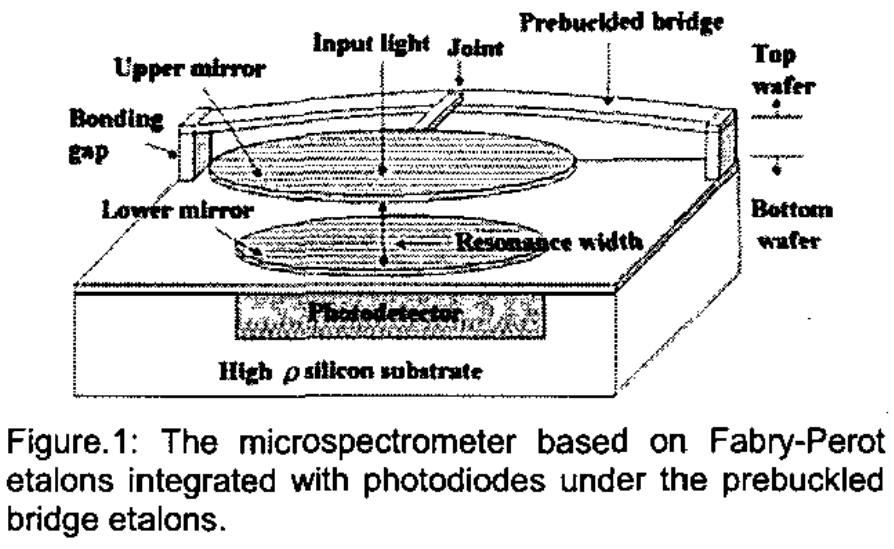
\includegraphics[width=.9\textwidth]{figures/A 16-channel array-type microspectrometer using integrated Fabry-Perot etalons and lateral pin photodetectors_1.png} %插入图片,[]中设置图片大小,{}中是图片文件名
                \caption{仪器结构示意图} %最终文档中希望显示的图片标题
            \end{figure}
            \begin{figure}[H] %H为当前位置,!htb为忽略美学标准,htbp为浮动图形
                \centering %图片居中
                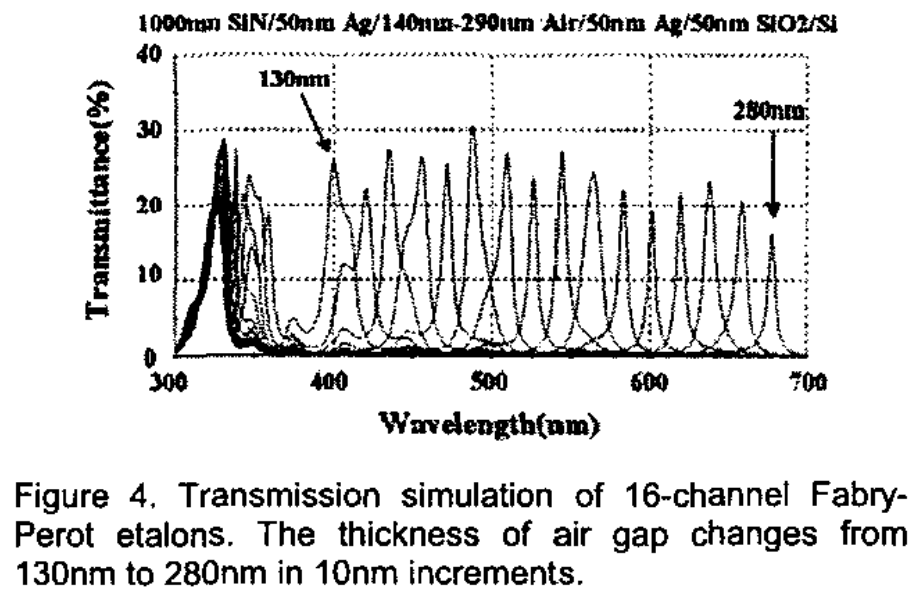
\includegraphics[width=.9\textwidth]{figures/A 16-channel array-type microspectrometer using integrated Fabry-Perot etalons and lateral pin photodetectors_2.png} %插入图片,[]中设置图片大小,{}中是图片文件名
                \caption{透射率关于波长} %最终文档中希望显示的图片标题
            \end{figure}
        \end{column}
    \end{columns}
\end{frame}

\begin{frame}[c]
    \frametitle{使用集成法布里-珀罗标准具和横向针式光电探测器的 16 通道阵列型显微光谱仪}
    \begin{itemize}
        \item 原文的膜结构:$1000 \mathrm{\ nm\ Si_3N_4} - 50 \mathrm{\ nm\ Ag} - 130\sim 280\mathrm{\ nm\ Air} - 50\mathrm{\ nm\ Ag} - 50\mathrm{\ nm\ SiO_2} - \mathrm{Si(substrate)}$
              \begin{itemize}
                  \item 其中顶层 $\mathrm{Si_3N_4}$ 是用来沉积 $\mathrm{Ag}$ 的。
                  \item 如果中间谐振腔由空气换为 $\mathrm{SiO_2}$,则无需这层 $\mathrm{Si_3N_4}$。
              \end{itemize}
        \item 改进后的膜结构:$100\mathrm{\ nm\ SiO_2} - 20 \mathrm{\ nm\ Ag} - 90\sim 200\mathrm{\ nm\ SiO_2} - 50\mathrm{\ nm\ Ag} - \mathrm{Si(substrate)}$
              \begin{itemize}
                  \item 考虑到外层的 $\mathrm{Ag}$ 容易被破坏,最外层附加 $\mathrm{100\ nm\ SiO_2}$ 作为保护。
              \end{itemize}
    \end{itemize}
    \begin{figure}[H] %H为当前位置,!htb为忽略美学标准,htbp为浮动图形
        \centering %图片居中
        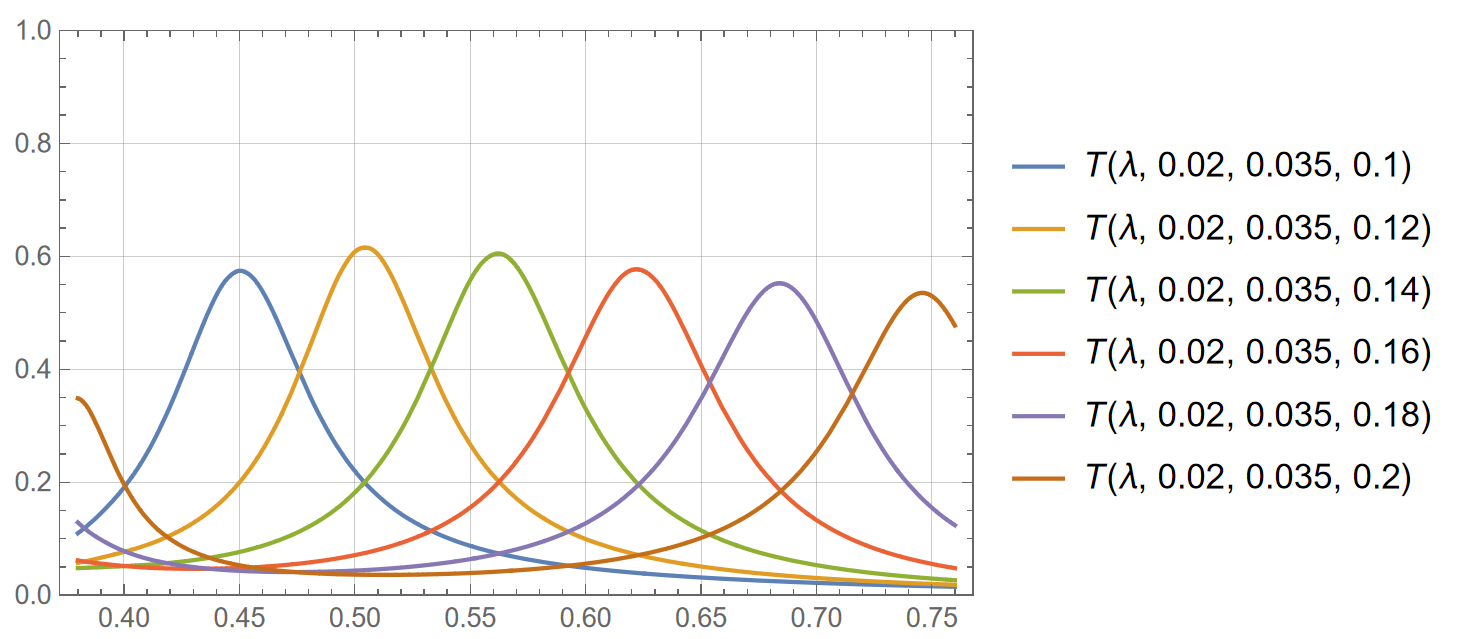
\includegraphics[width=.7\textwidth]{figures/A 16-channel array-type microspectrometer using integrated Fabry-Perot etalons and lateral pin photodetectors_3.png} %插入图片,[]中设置图片大小,{}中是图片文件名
        \caption{“改进后的膜结构”} %最终文档中希望显示的图片标题
    \end{figure}

    \begin{itemize}
        \item 若继续增加中间层 $\mathrm{SiO_2}$ 的厚度,透射峰将会出现在近红外区域,但是此时可见光短波处将会出现次级透射峰,该处的透射光将会造成较大的噪声。
    \end{itemize}
\end{frame}